%!TEX root = ../main.tex
\section{Politische Debatte}
  \subsection{Standpunkte einzelner Parteien}
        \begin{frame}<beamer>{Abstimmungsverhalten im Deutschen Bundestag}
\begin{itemize}
        \item Abstimmungsverhalten bei der Einführung der VDS
        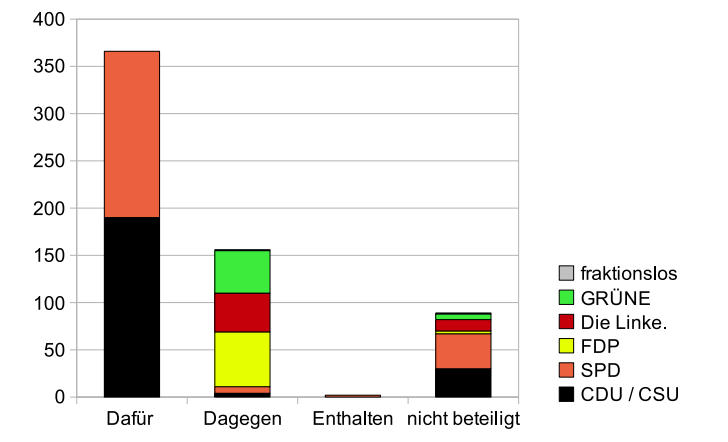
\includegraphics[height=1\textheight]{sections/img/abstimmung.png}
    \end{itemize}
    \end{frame}
  
  
    \begin{frame}<beamer>{Standpunkte der CDU}
       \begin{itemize}
        \item todo
  
      \end{itemize}
    \end{frame}

  \begin{frame}<beamer>{Standpunkte der SPD}
       \begin{itemize}
        \item todo
  
      \end{itemize}
    \end{frame}
    
    \begin{frame}<beamer>{Standpunkte der Grünen}
       \begin{itemize}
        \item todo
  
      \end{itemize}
    \end{frame}

    \begin{frame}<beamer>{Standpunkte der Linken}
       \begin{itemize}
        \item todo
  
      \end{itemize}
    \end{frame}

    \begin{frame}<beamer>{Standpunkte der FPD}
       \begin{itemize}
        \item todo
  
      \end{itemize}
    \end{frame}
      \subsection{Protestbewegungen}
    \begin{frame}<beamer>{Protestbewegungen}
       \begin{itemize}
        \item todo
  
      \end{itemize}
    \end{frame}


